\section{Signal Monitoring: noise removal}
\label{section:signal}

\paragraph{Method.} We compare a standard 0.5--40~Hz band-pass filter with a convolutional denoising autoencoder, a neural network that learns to map a noisy segment to the clean one \cite{chiang2019noise}. Our autoencoder compresses 1.4-second segments with three convolution layers and reconstructs them with three transposed convolutions. It is trained on segments from the training patients mixed with noise from the first half of each noise recording, at random signal-to-noise ratios between $-6$ and 18~dB. Testing uses the test patients and the second half of the noise recordings, so neither the patients nor the noise are seen in training. We measure the improvement in signal-to-noise ratio (SNR).

\begin{table}[H]
\caption{SNR improvement (dB) on the test patients; higher is better, best per row in bold.}
\label{tab:denoising}
\centering
\small
\setstretch{1.1}
\begin{tabular}{@{}llrr@{}}
\toprule
\textbf{Noise type} & \textbf{Input SNR} & \textbf{Band-pass filter} & \textbf{Autoencoder} \\
\midrule
Baseline wander & 0 dB & \textbf{12.4} & 9.8 \\
 & 6 dB & \textbf{10.4} & 5.3 \\
 & 12 dB & \textbf{7.6} & 0.1 \\
\addlinespace
Electrode motion & 0 dB & 1.6 & \textbf{7.2} \\
 & 6 dB & 1.3 & \textbf{3.8} \\
 & 12 dB & \textbf{0.6} & $-0.7$ \\
\addlinespace
Muscle artefact & 0 dB & 4.8 & \textbf{9.0} \\
 & 6 dB & 4.3 & \textbf{4.9} \\
 & 12 dB & \textbf{2.9} & 0.1 \\
\bottomrule
\end{tabular}
\end{table}

\begin{figure}[H]
\centering
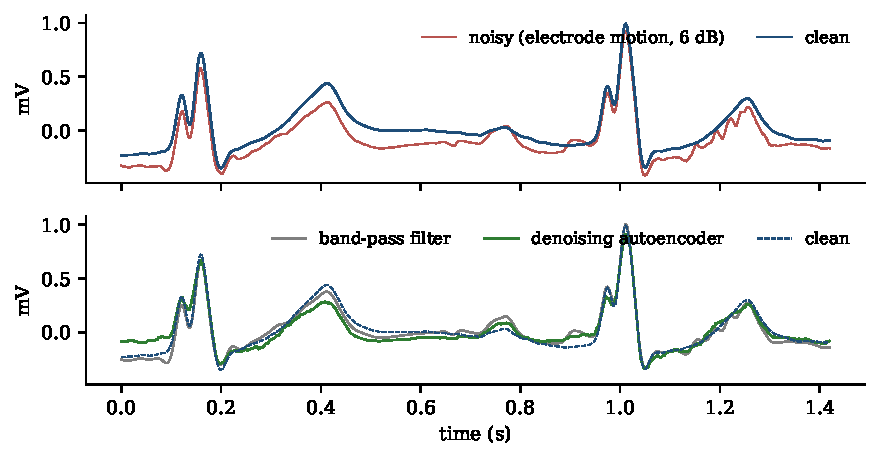
\includegraphics[width=0.8\textwidth]{Fig/s4_denoising_example.pdf}
\caption{Electrode-motion noise at 6~dB on a test patient (top), and the output of both methods (bottom).}
\label{fig:denoising}
\end{figure}

\paragraph{Results.} The two methods are complementary (Table~\ref{tab:denoising}). The band-pass filter is best for baseline wander, which lies mostly below its pass band. The autoencoder is much better for strong electrode-motion and muscle noise, which overlap with the ECG in frequency and which a fixed filter cannot remove: at 0~dB it gains 7.2~dB on electrode motion, against 1.6~dB for the filter (Figure~\ref{fig:denoising}). On mildly noisy signals (12~dB), however, the autoencoder adds small distortions of its own. The next version will therefore filter first and apply the autoencoder only when the signal-quality check reports strong noise.
